\documentclass{ctexbeamer}

\usepackage{filecontents}
\usepackage{graphicx}

% Use classyslides theme and pass options
\usetheme[%
  fonts%
  , colors=dark%
]{classyslides}

\mode<presentation>

\title{Linux入门}
\author[sunday]{sunday \\ synchronized@yeah.net}
\date{\today}

% Bibliography
% \begin{filecontents}{euclid.bib}
%   @book{Labov1972,
%     Address = {Philadelphia},
%     Author = {William Labov},
%     Publisher = {University of Pennsylvania Press},
%     Title = {Sociolinguistic Patterns},
%     Year = {1972}}
%
% @book{Chomsky1957,
%     Address = {The Hague},
%     Author = {Noam Chomsky},
%     Publisher = {Mouton},
%     Title = {Syntactic Structures},
%     Year = {1957}}
% }
%
% @online{wikipedia-euclid,
%   url={https://upload.wikimedia.org/wikipedia/commons/3/30/Euklid-von-Alexandria_1.jpg},
%   urldate={2018-10-22}
% }
%
% @online{wikipedia:sieve,
%   url={https://en.wikipedia.org/wiki/Sieve_of_Eratosthenes},
%   urldate={2018-10-29}
% }
% \end{filecontents}
% \addbibresource{./euclid.bib}

%
% Document
%
\begin{document}

\frame{
\titlepage
}

%! Table of contents.

\frame{
  \frametitle{大纲}
  \tableofcontents
}

\section{Unix与Linux发展史}
% \frame{
%   \sectionpage
% }
\begin{frame}
    \frametitle{Unix与Linux发展}
    \begin{itemize}
    \item 1965年,美国麻省理工学院(MIT),通用电器公司(GE),AT&T旗下贝尔实验室联
        合开发Multics工程计划,其目的是开发一种交互式具有多道处理程序处理能力
        的分时操作系统,但因Multics追求的目标过于庞大复杂,项目进度远远落后于
        计划,最后贝尔实验室宣布退出.
    \item 1969年,美国贝尔实验室的肯-汤姆森在DEC公司 PDP-7机器上开发出了
        Unix(Unics)系统,由于贝尔实验室推出了Multics项目,无法再使用该系统,早
        期在Multics上开发的游戏(Space Travel)无法运行,由此Unix诞生
    \end{itemize}
\end{frame}
\begin{frame}
    \frametitle{Unix与Linux发展}
    \begin{itemize}
    \item 1971年,肯-汤姆森的同事丹尼斯-里奇发明C语言,
        贝尔实验室,需要开发文字处理程序--nroff,肯-汤姆森负责nroff开发,
        由此Unix不断被改进
    \item 1972年,贝尔实验室, 10台Unix
    \item 1973年,Unix系统的绝大部分源代码用C语言重写,这为提高Unix系统的可移植性
        打下了基础
    \end{itemize}
\end{frame}
\begin{frame}
    \frametitle{Unix与Linux发展}
    \begin{itemize}
    \item 1974年,两人在《美国计算机通信》杂志上发表论文,介绍Unix
        随后各大高校,研究机构纷纷研究Unix,在其基础上开发,并且反馈给贝尔实验室
    \item 1976年,肯-汤姆森在年休期间到伯克利(Berkeley)任教
        Bill Joy 成立BSRG(Berkeley System Research Group),
    \item 1977年,BSRG发布BSD(Berkeley System Distribution)
    \end{itemize}
\end{frame}
\begin{frame}
    \frametitle{Unix与Linux发展}
    \begin{itemize}
    \item 1978年,SCO公司(第一家)公开发售商业版本Unix和商业版本C编译器
    \item 1979年,System v7 发布
    \item 1980年,美国国防部高级研究计划局(DARPA)研究tcp/ip
    \end{itemize}
\end{frame}
\begin{frame}
    \frametitle{Unix与Linux发展}
    \begin{itemize}
    \item 1982年,Bill Joy 成立SUN(Sun Microsystems)
        workstation(BSD)
    \item 1983年,tcp/ip协议诞生
    \item 1983年,DEC公司取消PDP-11之后的工作站,主打VAX
        VAX上本来预装的是本公司开发的系统(VMS)
        在市场环境下改为预装Unix
    \end{itemize}
\end{frame}
\section{苹果公司发展史}
\begin{frame}
    \frametitle{苹果公司发展史}
    \begin{itemize}
    \item 1976年,苹果公司成立,
    \item 1983年,苹果公司推出新型电脑Apple Lisa(图形界面)
    \end{itemize}
\end{frame}
\section{Microsoft发展史}
\begin{frame}
    \frametitle{Microsoft发展史}
    \begin{itemize}
    \item 1980年,Microsoft成立,只有两个款产品,Unix(XENIX)和basic编译器
    \item 1981年,Micorsoft, Bill Gates
        QDOS(Quick and Dirty Operating System)
    \end{itemize}
\end{frame}


\section{Linux组成}

\begin{frame}[allowframebreaks]
  \frametitle{What Are Prime Numbers?}
  \begin{Definition}{Prime number}
    A \emph{prime number} is a number that has exactly two divisors.
  \end{Definition}
  \framebreak
  \begin{Example}
    \begin{itemize}
      \item 2 is prime (two divisors: 1 and 2).
      \item 3 is prime (two divisors: 1 and 3).
      \item 4 is not prime (\alert{three} divisors: 1, 2, and 4).
    \end{itemize}
  \end{Example}
\end{frame}

\begin{frame}[fragile]
  \frametitle{There Is No Largest Prime Number}%
  \begin{Theorem}{Prime numbers}
    There is no largest prime number.
  \end{Theorem}
\end{frame}

\begin{frame}[fragile]
  \frametitle{There Is No Largest Prime Number}%
  \begin{Proof}
    \begin{enumerate}
      \item<1-> Suppose $p$ were the largest prime number.
      \item<2-> Let $q$ be the product of the first $p$ numbers.
      \item<3-> Then $q + 1$ is not divisible by any of them.
      \item<4-> But $q + 1$ is greater than $1$, thus divisible by some prime number not in the first $p$ numbers.\qedhere
    \end{enumerate}
  \end{Proof}
  \uncover<4->{The proof used \textit{reductio ad absurdum}.}
\end{frame}

\begin{frame}[t]
  \frametitle{What's Still To Do?}
  \begin{itemize}
    \item Answered Questions
    \begin{itemize}
      \item How many primes are there?
    \end{itemize}
    \item Open Questions
    \begin{itemize}
      \item Is every even number the sum of two primes?
    \end{itemize}
  \end{itemize}
\end{frame}

\begin{frame}[fragile, allowframebreaks]
  \frametitle{An Algorithm For Finding Prime Numbers.}
  \begin{Code}{FindPrimeNumbers}
Input: an integer n > 1.

Let A be an array of Boolean values, indexed by integers 2 to n,
initially all set to true.

for i = 2, 3, 4, ..., not exceeding $\sqrt n$:
  if A[i] is true:
    for j = i2, i2+i, i2+2i, i2+3i, ..., not exceeding n:
      A[j] := false.

Output: all i such that A[i] is true.
  \end{Code}
  cf. \cite{wikipedia:sieve}
\end{frame}

\frame{
  \frametitle{It's me, Euclid}
  \begin{figure}
    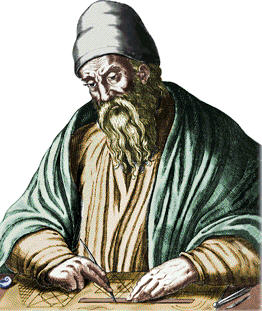
\includegraphics[height=0.6\textheight]{./euclid.jpg}
    \caption{It's me, Euclid \cite{wikipedia-euclid}}
  \end{figure}
}

\nocite{*}
\begin{frame}[allowframebreaks]
  \frametitle{References}
  \printbibliography
\end{frame}
\end{document}
